% Provenance (never printed): see sources/outline_sources.md (Year 3:
% critical-taper theory; fold-and-thrust belts; exhumation and
% thermochronology). Brief: sources/book5/BRIEFS.md, ch. 10. Curves from
% figdata/bachelor-3/fault_bend.py, critical_taper.py and age_elevation.py.
% Exercise and problem values in the Book 5 scratch calculator calc/ch10.py.
\chapter{Sabuk Sesar Dorong dan Baji Orogen}\label{ch:b3:orogenic-wedges}

Dorong sebuah buldoser ke dalam pasir basah atau salju, dan sebuah baji material menumpuk
di depan bilahnya. Ia berdeformasi hingga permukaannya mencapai kemiringan tertentu;
sejak saat itu ia meluncur ke depan sebagai satu kesatuan dan tumbuh dengan bentuk yang sama,
dengan menyerap material baru di ujung depannya. Bagian luar sabuk pegunungan, dari
Taiwan hingga kaki bukit Alpen, berperilaku dengan cara yang sama: keduanya berupa baji
batuan yang dikerok dari sebuah lempeng dan didorong di atas dasar yang lemah, dan
kemiringan permukaan serta kemiringan dasarnya menunjukkan seberapa lemah dasar itu dan seberapa tinggi
tekanan fluida di dalamnya. Bab ini membahas geometri sabuk sesar dorong, mekanika baji,
serta jam-jam yang mengukur seberapa cepat
batuannya naik ke permukaan.
% ledger: dsd83:taper

\begin{recall}
Sesar dorong, vergensi, dan geometri lipatan dibahas dalam volume Tahun 1, pada bab
tentang sesar, lipatan, dan fabrik; kriteria Coulomb, hukum Byerlee, serta
tegangan efektif dan rasio tekanan pori $\lambda = P/\sigma_v$ dalam
bab tentang tegangan, regangan, dan reologi; suhu penutupan dan umur pendinginan
dalam bab tentang metode penanggalan radiometrik. Décollement, sabuk lipatan-dan-sesar dorong,
tektonik kulit tipis dan kulit tebal, serta
penampang seimbang dibahas di volume Tahun 2, pada bab tentang anatomi sebuah
sabuk pegunungan; ekshumasi dan laju ekshumasinya pada bab tentang lintasan P--T--t. Konstruksi
kink dan luas berlebih $A = Sh$ dari lipatan di atas detasemen
dibahas dalam \cref{ch:b3:structural-analysis}; \omterm{def:b3:lithosphere-thermal-models:peclet}{bilangan Péclet termal} pada
\cref{ch:b3:lithosphere-thermal-models}.
\end{recall}

\section{Geometri sesar dorong}\label{sec:b3:orogenic-wedges:geometry}

Sesar dorong tidak memotong urutan berlapis sepanjang satu bidang lurus.
Ia mengikuti lapisan lemah, berupa serpih atau evaporit, untuk jarak yang panjang, lalu
naik curam melalui lapisan kuat di atasnya hingga lapisan lemah berikutnya. Bentuk
tangga yang ditorehkannya mengendalikan lipatan pada dinding gantung.

\begin{definition}[Tanjakan, bagian datar, dupleks, sesar dorong luar-urutan]\label{def:b3:orogenic-wedges:thrust-geometry}
Yang disebut \emph{bagian datar}\index{bagian datar} adalah segmen sesar dorong yang berjalan
sejajar dengan perlapisan, biasanya pada lapisan lemah; sebuah \emph{tanjakan}\index{tanjakan}
adalah segmen yang memotong perlapisan,
biasanya pada sudut 20 hingga \ang{30}, yang menghubungkan bagian datar bawah dengan bagian datar atas. Yang disebut
\emph{dupleks}\index{dupleks} adalah tumpukan irisan yang dibatasi sesar,
yaitu kuda, yang terapit di antara sesar dorong lantai di bawah dan sesar dorong atap di atas,
setiap kuda dipotong oleh tanjakan yang menghubungkan keduanya. Sesar dorong umumnya terbentuk
secara berurutan, masing-masing yang baru berada di dinding bawah sesar sebelumnya, lebih dekat ke
depan-pegunungan; sebuah \emph{sesar dorong luar-urutan}\index{sesar dorong luar-urutan} adalah
satu yang terbentuk atau tergelincir lagi di belakang front aktif, memotong sesar dorong yang lebih tua.
\end{definition}

Ketika dinding gantung bergerak melewati tekukan pada sesar, ia harus terlipat agar tetap
bersentuhan dengan sesar: sinklin terbentuk di tempat ia masuk ke \omterm{def:b3:orogenic-wedges:thrust-geometry}{tanjakan}, dan
antiklin terbentuk di tempat ia meninggalkannya.

\begin{definition}[Lipatan tekukan-sesar, lipatan propagasi-sesar, dan lipatan detasemen]\label{def:b3:orogenic-wedges:thrust-folds}
Yang disebut \emph{lipatan tekukan-sesar}\index{lipatan tekukan-sesar} adalah lipatan pada dinding gantung
sesar dorong yang terbentuk ketika meluncur melewati tekukan sesar, yaitu \omterm{def:b3:orogenic-wedges:thrust-geometry}{tanjakan} di antara
dua \omterm{def:b3:orogenic-wedges:thrust-geometry}{bagian datar}. Yang disebut \emph{lipatan propagasi-sesar}\index{lipatan propagasi-sesar}
tumbuh di atas ujung sesar dorong yang masih merambat ke atas: pemendekan yang
tidak lagi ditanggung sesar diserap oleh pelipatan di depan
ujungnya, sehingga menghasilkan sayap depan yang curam atau terbalik. Yang disebut
\emph{lipatan detasemen}\index{lipatan detasemen} tumbuh di atas \omterm{def:b3:orogenic-wedges:thrust-geometry}{bagian datar} tanpa \omterm{def:b3:orogenic-wedges:thrust-geometry}{tanjakan}: pemendekan
diserap oleh pelipatan dan oleh lapisan lemah, garam atau serpih, yang mengalir masuk ke
intinya.
\end{definition}

Gambar di bawah membangun sebuah \omterm{def:b3:orogenic-wedges:thrust-folds}{lipatan tekukan-sesar}. Di sini dinding gantung bergerak
sejajar dengan segmen sesar di bawahnya dan terlipat pada bidang aksial yang
membagi dua setiap tekukan, sebuah model kinematik yang disebut aliran sejajar-sesar;
model klasik dengan ketebalan dan panjang lapisan tetap menghasilkan antiklin berpuncak datar
dengan sayap depan yang lebih curam, dengan konsekuensi konstruksi yang lebih panjang
(diakui di sini). Kedua model terikat oleh kekekalan luas.

\begin{omfigure}
\begin{tikzpicture}
\begin{groupplot}[group style={group size=1 by 2, vertical sep=0.9cm},
  width=0.92\linewidth, axis equal image,
  xmin=0, xmax=12, ymin=-0.6, axis lines=none, clip=true,
  title style={font=\small, at={(0.0,1.0)}, anchor=south west}]
% (a) before slip
\nextgroupplot[title={(a) sebelum geser}, ymax=1.75]
\fill[omLithSand!70] (axis cs:0,0) rectangle (axis cs:12,1.6);
\fill[gray!25] (axis cs:0,-0.6) rectangle (axis cs:12,0);
\draw[black!70] (axis cs:0,0.25) -- (axis cs:12,0.25);
\draw[black!70] (axis cs:0,0.5) -- (axis cs:12,0.5);
\draw[black!70] (axis cs:0,0.75) -- (axis cs:12,0.75);
\draw[black!70] (axis cs:0,1.0) -- (axis cs:12,1.0);
\draw[black!70] (axis cs:0,1.3) -- (axis cs:12,1.3);
\draw[black!70] (axis cs:0,1.6) -- (axis cs:12,1.6);
\draw[black!70] (axis cs:0,-0.3) -- (axis cs:12,-0.3);
\addplot[very thick, red!70!black] table[x=x, y=y] {figdata/out/bachelor-3-fault_bend-fault.dat};
\node[font=\scriptsize, fill=omLithSand!70, inner sep=1pt] at (axis cs:2,0.125) {bagian datar bawah};
\node[font=\scriptsize, fill=omLithSand!70, inner sep=1pt, rotate=30] at (axis cs:4.55,0.62) {tanjakan};
\node[font=\scriptsize, fill=omLithSand!70, inner sep=1pt] at (axis cs:9,0.875) {bagian datar atas};
% (b) after a slip of 2.5 units
\nextgroupplot[title={(b) setelah geser: sebuah lipatan tekukan-sesar}, ymax=2.75]
\fill[gray!25] (axis cs:0,-0.6) rectangle (axis cs:12,0) -- cycle;
\addplot[name path=fault, draw=none] table[x=x, y=y] {figdata/out/bachelor-3-fault_bend-fault.dat};
\addplot[name path=top, draw=none] table[x=x, y=y] {figdata/out/bachelor-3-fault_bend-bed6.dat};
\addplot[name path=base, draw=none] coordinates {(0,-0.6) (12,-0.6)};
\addplot[omLithSand!70] fill between[of=fault and top];
\addplot[gray!25] fill between[of=base and fault];
\addplot[black!70] table[x=x, y=y] {figdata/out/bachelor-3-fault_bend-bed1.dat};
\addplot[black!70] table[x=x, y=y] {figdata/out/bachelor-3-fault_bend-bed2.dat};
\addplot[black!70] table[x=x, y=y] {figdata/out/bachelor-3-fault_bend-bed3.dat};
\addplot[black!70] table[x=x, y=y] {figdata/out/bachelor-3-fault_bend-bed4.dat};
\addplot[black!70] table[x=x, y=y] {figdata/out/bachelor-3-fault_bend-bed5.dat};
\addplot[black!70] table[x=x, y=y] {figdata/out/bachelor-3-fault_bend-bed6.dat};
\draw[black!70] (axis cs:4.4330,0.25) -- (axis cs:12,0.25);
\draw[black!70] (axis cs:4.8660,0.5) -- (axis cs:12,0.5);
\draw[black!70] (axis cs:5.2990,0.75) -- (axis cs:12,0.75);
\draw[black!70] (axis cs:0,-0.3) -- (axis cs:12,-0.3);
\addplot[very thick, red!70!black] table[x=x, y=y] {figdata/out/bachelor-3-fault_bend-fault.dat};
\draw[densely dashed, black!60] (axis cs:0,1.6) -- (axis cs:12,1.6);
\node[font=\scriptsize, anchor=south] at (axis cs:2.2,1.65) {regional};
\node[font=\scriptsize, anchor=west] at (axis cs:8.6,2.25) {luas berlebih $A = Sr$};
\draw[black!70] (axis cs:8.6,2.25) -- (axis cs:6.6,2.0);
\node[font=\scriptsize, fill=gray!25, inner sep=1pt] at (axis cs:10.6,0.625) {dinding bawah};
\end{groupplot}
\end{tikzpicture}

\par\smallskip{\small (a) Sesar dorong dengan \omterm{def:b3:orogenic-wedges:thrust-geometry}{bagian datar} bawah, \omterm{def:b3:orogenic-wedges:thrust-geometry}{tanjakan} yang miring
\ang{30}, dan \omterm{def:b3:orogenic-wedges:thrust-geometry}{bagian datar} atas, sebelum slip (skematis, skala vertikal dan horizontal
sama). (b) Keadaan yang sama setelah slip sebesar 2.5 kali tinggi \omterm{def:b3:orogenic-wedges:thrust-geometry}{tanjakan}, dihitung
dengan aliran sejajar sesar: sinklin di kaki \omterm{def:b3:orogenic-wedges:thrust-geometry}{tanjakan}, sayap belakang
yang sejajar dengan \omterm{def:b3:orogenic-wedges:thrust-geometry}{tanjakan}, puncak datar yang terangkat sejauh tinggi \omterm{def:b3:orogenic-wedges:thrust-geometry}{tanjakan} $r$, sayap
depan, dan luas berlebih $Sr$ di atas level regional setiap lapisan di atas
\omterm{def:b3:orogenic-wedges:thrust-geometry}{bagian datar} atas.}\label{fig:b3:orogenic-wedges:thrusts}
\end{omfigure}


\begin{proposition}[Luas berlebih lipatan tekukan-sesar]\label{prop:b3:orogenic-wedges:fault-bend-area}
Misalkan sesar dorong membawa dinding gantungnya naik melalui \omterm{def:b3:orogenic-wedges:thrust-geometry}{tanjakan} setinggi $r$ dari \omterm{def:b3:orogenic-wedges:thrust-geometry}{bagian datar} bawah
ke \omterm{def:b3:orogenic-wedges:thrust-geometry}{bagian datar} atas, dengan slip $S$ pada \omterm{def:b3:orogenic-wedges:thrust-geometry}{bagian datar} bawah. Untuk setiap lapisan dinding gantung
yang berada di atas \omterm{def:b3:orogenic-wedges:thrust-geometry}{bagian datar} atas, luas yang dibatasi antara lapisan
terlipat dan level awalnya bernilai $A = Sr$, sama untuk setiap lapisan seperti itu.
\end{proposition}

\begin{proof}
Batuan tidak diciptakan maupun dimusnahkan, dan volumenya tetap. Ambil irisan
sejajar slip, dibatasi dua garis vertikal yang jauh di belakang dan jauh di depan
\omterm{def:b3:orogenic-wedges:thrust-geometry}{tanjakan}. Melalui garis belakang, dinding gantung di antara \omterm{def:b3:orogenic-wedges:thrust-geometry}{bagian datar} bawah
dan sebuah lapisan pada ketinggian $y_0$ di atasnya telah bergerak masuk sejauh $S$: luas
$Sy_0$ telah masuk. Melalui garis depan, batuan di antara \omterm{def:b3:orogenic-wedges:thrust-geometry}{bagian datar} atas
dan lapisan yang sama, dengan tebal $y_0 - r$, telah bergerak keluar sejauh slip pada
\omterm{def:b3:orogenic-wedges:thrust-geometry}{bagian datar} atas, juga $S$ bila batuan mempertahankan luasnya: luas $S(y_0 - r)$
telah keluar. Selisihnya, $Sr$, tetap berada di antara kedua garis, dan mengangkat
lapisan di atas level awalnya.
\end{proof}

Luas berlebih \omterm{def:b3:orogenic-wedges:thrust-folds}{lipatan tekukan-sesar} mengukur slip dikali tinggi
\omterm{def:b3:orogenic-wedges:thrust-geometry}{tanjakan}, bukan dikali kedalaman ke décollement, seperti yang berlaku untuk
\omterm{def:b3:orogenic-wedges:thrust-folds}{lipatan detasemen} (lihat \cref{ch:b3:structural-analysis}). Kedua jenis lipatan
harus dibedakan sebelum luas diubah menjadi pemendekan.


\omterm{def:b3:orogenic-wedges:thrust-geometry}{Dupleks} (gambar di bawah) tumbuh ketika sesar dorong, alih-alih terus membawa dinding gantungnya
lebih jauh sepanjang \omterm{def:b3:orogenic-wedges:thrust-geometry}{tanjakan} yang sama, meninggalkannya dan memotong \omterm{def:b3:orogenic-wedges:thrust-geometry}{tanjakan} baru di dinding bawahnya,
di depan \omterm{def:b3:orogenic-wedges:thrust-geometry}{tanjakan} lama. Irisan di antara \omterm{def:b3:orogenic-wedges:thrust-geometry}{tanjakan} lama dan baru menjadi
kuda, dibawa naik melalui \omterm{def:b3:orogenic-wedges:thrust-geometry}{tanjakan} baru dan ditumpuk di bawah atap; \omterm{def:b3:orogenic-wedges:thrust-geometry}{tanjakan} berikutnya
terbentuk lagi di depan. Setiap kuda dipendekkan dari panjang awalnya menjadi
panjang yang kini ditempatinya sepanjang lantai, dan pemendekan \omterm{def:b3:orogenic-wedges:thrust-geometry}{dupleks} adalah
jumlah seluruh kudanya. \omterm{def:b3:orogenic-wedges:thrust-geometry}{Sesar dorong luar-urutan} memotong urutan ini: terbentuk
ketika baji di belakang front harus menebal, kasus yang diprediksi oleh mekanika
subbab berikutnya.

\begin{omfigure}
\begin{tikzpicture}
\begin{axis}[width=0.92\linewidth, axis equal image, xmin=0, xmax=12, ymin=-0.6, ymax=1.95,
  axis lines=none, clip=true]
\fill[gray!25] (axis cs:0,-0.6) rectangle (axis cs:12,0);
\fill[omLithSand!70] (axis cs:0,0) -- (axis cs:1.0,0) -- (axis cs:2.35,1.15) -- (axis cs:12,1.15) -- (axis cs:12,1.85) -- (axis cs:2.35,1.85) -- (axis cs:1.0,0.7) -- (axis cs:0,0.7) -- cycle;
\draw[black!70] (axis cs:0,0.35) -- (axis cs:1.0,0.35) -- (axis cs:2.35,1.5) -- (axis cs:12,1.5);
\draw[black!70] (axis cs:0,0.7) -- (axis cs:1.0,0.7) -- (axis cs:2.35,1.85) -- (axis cs:12,1.85);
\fill[omLithShale!60] (axis cs:8.2,0) -- (axis cs:12,0) -- (axis cs:12,1.15) -- (axis cs:9.55,1.15) -- cycle;
\draw[black!70] (axis cs:8.646,0.38) -- (axis cs:12,0.38);
\draw[black!70] (axis cs:9.104,0.77) -- (axis cs:12,0.77);
\fill[omLithLime] (axis cs:1.0,0) -- (axis cs:2.80,0) -- (axis cs:4.15,1.15) -- (axis cs:2.35,1.15) -- cycle;
\draw[black!70] (axis cs:1.45,0) -- (axis cs:2.80,1.15);
\draw[black!70] (axis cs:1.90,0) -- (axis cs:3.25,1.15);
\draw[black!70] (axis cs:2.35,0) -- (axis cs:3.70,1.15);
\fill[omLithShale] (axis cs:2.8,0) -- (axis cs:4.60,0) -- (axis cs:5.95,1.15) -- (axis cs:4.15,1.15) -- cycle;
\draw[black!70] (axis cs:3.25,0) -- (axis cs:4.60,1.15);
\draw[black!70] (axis cs:3.70,0) -- (axis cs:5.05,1.15);
\draw[black!70] (axis cs:4.15,0) -- (axis cs:5.50,1.15);
\fill[omLithLime] (axis cs:4.6,0) -- (axis cs:6.40,0) -- (axis cs:7.75,1.15) -- (axis cs:5.95,1.15) -- cycle;
\draw[black!70] (axis cs:5.05,0) -- (axis cs:6.40,1.15);
\draw[black!70] (axis cs:5.50,0) -- (axis cs:6.85,1.15);
\draw[black!70] (axis cs:5.95,0) -- (axis cs:7.30,1.15);
\fill[omLithShale] (axis cs:6.4,0) -- (axis cs:8.20,0) -- (axis cs:9.55,1.15) -- (axis cs:7.75,1.15) -- cycle;
\draw[black!70] (axis cs:6.85,0) -- (axis cs:8.20,1.15);
\draw[black!70] (axis cs:7.30,0) -- (axis cs:8.65,1.15);
\draw[black!70] (axis cs:7.75,0) -- (axis cs:9.10,1.15);
\draw[thick, red!70!black] (axis cs:1.0,0) -- (axis cs:2.35,1.15);
\draw[thick, red!70!black] (axis cs:2.8,0) -- (axis cs:4.15,1.15);
\draw[thick, red!70!black] (axis cs:4.6,0) -- (axis cs:5.95,1.15);
\draw[thick, red!70!black] (axis cs:6.4,0) -- (axis cs:7.75,1.15);
\draw[thick, red!70!black] (axis cs:8.2,0) -- (axis cs:9.55,1.15);
\draw[very thick, red!70!black] (axis cs:0,0) -- (axis cs:12,0);
\draw[very thick, red!70!black] (axis cs:2.35,1.15) -- (axis cs:12,1.15);
\node[font=\scriptsize, anchor=north west] at (axis cs:0.1,-0.04) {sesar dorong dasar};
\node[font=\scriptsize, anchor=south west] at (axis cs:7.0,1.17) {sesar dorong atap};
\node[font=\scriptsize, anchor=north] at (axis cs:5.6,-0.12) {kuda};
\draw[black!70] (axis cs:5.6,-0.15) -- (axis cs:5.5,0.45);
\draw[->, thick] (axis cs:0.15,0.52) -- (axis cs:0.95,0.52);
\end{axis}
\end{tikzpicture}

\par\smallskip{\small \omterm{def:b3:orogenic-wedges:thrust-geometry}{Dupleks} (skematis): empat kuda (biru dan hijau) terpotong
oleh \omterm{def:b3:orogenic-wedges:thrust-geometry}{tanjakan} di antara sesar dorong dasar dan sesar dorong atap, di depannya dinding bawah belum
terpotong, panah menunjukkan arah transpor; batuan penutup di atas atap
terlipat di atas tumpukan.}\label{fig:b3:orogenic-wedges:duplex}
\end{omfigure}


\section{Taper kritis}\label{sec:b3:orogenic-wedges:taper}

Sabuk lipatan-dan-sesar dorong dalam penampang melintang adalah baji: tipis di frontnya, tempat
décollement mencapai permukaan, dan menebal ke arah belakang-pegunungan.
Permukaan atasnya miring ke arah depan-pegunungan dengan sudut $\alpha$; alasnya,
yaitu décollement, miring ke arah belakang-pegunungan dengan sudut $\beta$. Taper
baji adalah sudut di antara keduanya, $\alpha + \beta$.

\begin{definition}[Taper kritis]\label{def:b3:orogenic-wedges:critical-taper}
\emph{Taper kritis}\index{taper kritis} dari baji yang didorong dari belakang
di atas suatu alas adalah taper ketika baji berada di seluruh bagiannya pada ambang
kegagalan, di dalam dan sepanjang alasnya, di bawah kompresi horizontal. Baji pada
taper kritisnya meluncur di atas alasnya tanpa berdeformasi di dalam; baji
di bawahnya (subkritis) berdeformasi dan menebal hingga mencapainya; baji
di atasnya (superkritis) meluncur tanpa berdeformasi.
\end{definition}
% ledger: dsd83:taper

\begin{omfigure}
\begin{tikzpicture}[>=stealth, x=1cm, y=1cm]
\fill[omLithSand!70] (0,0) -- (10,-1.05) -- (10,1.4) -- cycle;
\fill[gray!25] (0,0) -- (10,-1.05) -- (10,-1.6) -- (-0.8,-1.6) -- (-0.8,0) -- cycle;
\draw[thick] (-0.8,0) -- (0,0) -- (10,1.4);
\draw[very thick, red!70!black] (0,0) -- (10,-1.05);
\fill[gray!60] (10,-1.6) rectangle (10.6,1.9);
\node[font=\scriptsize, rotate=90] at (10.3,0.15) {penahan};
\draw[dashed] (0,0) -- (2.6,0);
\draw (2.2,0) arc[start angle=0, end angle=8, radius=2.2];
\node[font=\small] at (2.45,0.2) {$\alpha$};
\draw (2.2,0) arc[start angle=0, end angle=-6, radius=2.2];
\node[font=\small] at (2.45,-0.2) {$\beta$};
% slice
\draw[thick, omDef] (5.5,-0.5775) -- (5.5,0.77);
\draw[thick, omDef] (6.5,-0.6825) -- (6.5,0.91);
\draw[->, thick, omDef] (4.5,0.05) -- (5.45,0.05);
\node[font=\scriptsize, anchor=east] at (4.5,0.05) {$F(x)$};
\draw[<-, thick, omDef] (6.55,0.1) -- (7.6,0.1);
\node[font=\scriptsize, anchor=west] at (7.6,0.1) {$F(x + \mathrm dx)$};
\draw[->, thick, omProp] (6.0,-0.63) -- (6.75,-0.71);
\node[font=\scriptsize, anchor=north] at (6.4,-0.75) {$\tau_b$};
\draw[->, thick, omProp] (6.0,-0.63) -- (6.1,0.0);
\node[font=\scriptsize, anchor=east] at (6.02,-0.22) {$\sigma_n$};
\node[font=\scriptsize] at (6.0,1.2) {irisan $\mathrm dx$};
\draw[->, thick] (1.8,-1.25) -- (0.6,-1.25);
\node[font=\scriptsize, anchor=west] at (1.85,-1.25) {transpor};
\node[font=\scriptsize, anchor=west] at (0.2,-0.42) {décollement};
\node[font=\scriptsize] at (8.9,-0.45) {baji};
\draw[->] (0.1,0.5) -- (0.4,0.5); \node[font=\scriptsize, anchor=east] at (0.1,0.5) {$x$};
\end{tikzpicture}

\par\smallskip{\small Baji dengan lereng permukaan $\alpha$ yang bertumpu pada
décollement dengan kemiringan $\beta$ dan didorong dari belakang; $x$ diukur dari
ujung depan ke arah belakang-pegunungan. Pada irisan vertikal, dorongan $F(x + \mathrm dx)$
dari belakang melampaui dorongan $F(x)$ dari depan sebesar yang ditahan alas:
yaitu gesekannya $\tau_b$ dan bagian horizontal tegangan normalnya $\sigma_n$,
yang condong ke arah belakang-pegunungan pada alas yang miring ke arah itu (skematis,
sudut dilebih-lebihkan).}\label{fig:b3:orogenic-wedges:wedge}
\end{omfigure}

\begin{theorem}[Persamaan taper kritis]\label{thm:b3:orogenic-wedges:critical-taper}
Tinjau baji subaerial dengan massa jenis seragam $\rho$ yang tersusun dari bahan
Coulomb tanpa kohesi dengan gesekan internal $\mu = \tan\phi$, dengan rasio tekanan
pori $\lambda$, di atas alas dengan gesekan $\mu_b$ dan rasio tekanan pori
$\lambda_b$. Jika $\alpha$ dan $\beta$ kecil dan $\sigma_1$ horizontal,
maka \emph{persamaan taper kritis}\index{persamaan taper kritis} adalah
\[
  \alpha + \beta = \frac{\beta + \mu_b(1 - \lambda_b)}{1 + K(1 - \lambda)},
  \qquad K = \frac{2\sin\phi}{1 - \sin\phi},
\]
dengan sudut dalam radian.
\end{theorem}

\begin{proof}
Misalkan $z$ adalah kedalaman di bawah permukaan. Untuk lereng kecil, tegangan vertikal
adalah berat batuan di atasnya, $\sigma_{zz} = \rho g z$, dan tekanan pori
adalah $\lambda\rho g z$, sehingga tegangan vertikal efektif adalah
$(1 - \lambda)\rho g z$. Di setiap titik pada kegagalan dengan $\sigma_1$ horizontal,
kriteria Coulomb untuk bahan tanpa kohesi memberikan \omterm{def:b3:structural-analysis:palaeostress}{rasio tegangan}
utama efektif $\sigma'_1/\sigma'_3 = (1 + \sin\phi)/(1 -
\sin\phi) = 1 + K$, sehingga tegangan horizontal total
\[
  \sigma_{xx} = (1 + K)(1 - \lambda)\rho g z + \lambda\rho g z
  = \bigl(1 + K(1 - \lambda)\bigr)\rho g z .
\]
Pada jarak $x$ dari ujung depan, baji memiliki tebal $H = (\alpha +
\beta)x$, dan gaya horizontal per satuan panjang sabuk pada penampang vertikal
adalah $F = \int_0^H \sigma_{xx}\,\mathrm dz = \bigl(1 + K(1 -
\lambda)\bigr)\rho g H^2/2$. Pada irisan di antara $x$ dan $x + \mathrm dx$
(lihat gambar di atas), permukaan tidak memikul tegangan dan dorongan dari belakang
melampaui dorongan dari depan sebesar $(\mathrm dF/\mathrm dx)\,\mathrm dx$.
Alas menahan irisan itu dengan dua cara: gesekan $\mu_b(1 -
\lambda_b)\rho g H$ per satuan panjang, dan tegangan normalnya $\rho g H$, yang
tegak lurus alas yang miring $\beta$ ke arah belakang-pegunungan sehingga
condong ke arah itu sebesar $\beta$, memberikan bagian horizontal $\beta\rho g H$.
Kesetimbangan irisan menuntut
\[
  \bigl(1 + K(1 - \lambda)\bigr)\rho g H(\alpha + \beta)
  = \bigl(\beta + \mu_b(1 - \lambda_b)\bigr)\rho g H ,
\]
yaitu persamaan tadi. Karena $H$ saling meniadakan, baji pada kegagalan
mempertahankan taper yang sama seiring pertumbuhannya.
\end{proof}

Persamaan ini menyatakan, pertama, bahwa taper ditentukan oleh rasio kekuatan
alas, di pembilang, terhadap kekuatan baji, di
penyebut: alas lemah menghasilkan baji tipis, alas kuat menghasilkan baji tebal.
Kedua, lereng permukaan turun seiring alas yang makin curam. Ketiga, tekanan fluida
menurunkan taper: menaikkan $\lambda = \lambda_b$ lebih banyak mengurangi
kekuatan alas, secara proporsional, daripada kekuatan
baji. Gambar di bawah menunjukkan lereng permukaan kritis untuk
koefisien gesekan yang dicocokkan di Taiwan barat. Titik di bawah setiap garis adalah baji subkritis
yang menebal; titik di atas adalah baji superkritis, yang meluncur.
% ledger: dsd83:taper

\begin{omfigure}
\begin{tikzpicture}
\begin{axis}[omrecord, width=0.8\linewidth, height=0.5\linewidth,
  xlabel={kemiringan alas $\beta$ (\unit{\degree})}, ylabel={lereng permukaan $\alpha$ (\unit{\degree})},
  xmin=0, xmax=15, ymin=0, ymax=12, legend style={font=\scriptsize, at={(0.98,0.98)},
  anchor=north east, legend cell align=left}]
% computed in figdata/bachelor-3/critical_taper.py
\addplot[name path=t3, draw=none, forget plot] table[x=beta, y=t3] {figdata/out/bachelor-3-critical_taper-bands.dat};
\addplot[name path=t4, draw=none, forget plot] table[x=beta, y=t4] {figdata/out/bachelor-3-critical_taper-bands.dat};
\addplot[name path=t12, draw=none, forget plot] table[x=beta, y=t12] {figdata/out/bachelor-3-critical_taper-bands.dat};
\addplot[name path=t13, draw=none, forget plot] table[x=beta, y=t13] {figdata/out/bachelor-3-critical_taper-bands.dat};
\addplot[omLithEvap, area legend] fill between[of=t3 and t4];
\addlegendentry{sudut taper 3--\ang{4} (Jura)}
\addplot[omLithLime, area legend] fill between[of=t12 and t13];
\addlegendentry{sudut taper 12--\ang{13}}
\addplot[omDef, thick] table[x=beta, y=a040] {figdata/out/bachelor-3-critical_taper-curves.dat};
\addlegendentry{$\lambda = 0.4$}
\addplot[red!70!black, thick, densely dashed] table[x=beta, y=a070] {figdata/out/bachelor-3-critical_taper-curves.dat};
\addlegendentry{$\lambda = 0.7$}
\addplot[black, thick, densely dotted] table[x=beta, y=a090] {figdata/out/bachelor-3-critical_taper-curves.dat};
\addlegendentry{$\lambda = 0.9$}
\node[font=\scriptsize] at (axis cs:2.2,1.1) {subkritis};
\node[font=\scriptsize] at (axis cs:1.6,8.6) {superkritis};
\end{axis}
\end{tikzpicture}

\par\smallskip{\small Kemiringan permukaan kritis terhadap kemiringan dasar untuk
koefisien gesekan Taiwan bagian barat, $\mu = 1.03$ di dalam dan $\mu_b =
0.85$ pada dasar, untuk tiga rasio tekanan pori $\lambda = \lambda_b$;
``subkritis'' dan ``superkritis'' merujuk ke garis $\lambda = 0.7$. Pita
berarsir adalah taper baji sesar dorong Jura, 3 sampai \ang{4}, dan
baji di selatannya, 12 sampai \ang{13}.}\label{fig:b3:orogenic-wedges:taper}
\end{omfigure}
% ledger: dsd83:taper, deville21:jura

Baji bukan objek statis: material ditambahkan kepadanya dan dikeluarkan darinya,
dan setiap perubahan mendorongnya keluar dari \omterm{def:b3:orogenic-wedges:critical-taper}{taper kritisnya}.

\begin{definition}[Akresi frontal, underplating tektonik]\label{def:b3:orogenic-wedges:accretion}
Yang disebut \emph{akresi frontal}\index{akresi frontal} adalah penambahan material
pada ujung baji, saat décollement merambat ke dalam sedimen yang belum
terdeformasi di depan-pegunungan, dan sebuah irisan sesar dorong baru terpotong. Yang disebut \emph{underplating
tektonik}\index{underplating tektonik} adalah penambahan material ke
dasar baji, di belakang ujungnya, ketika irisan lempeng bawah
terlepas dan ditumpuk di bawahnya, sering kali sebagai \omterm{def:b3:orogenic-wedges:thrust-geometry}{dupleks}.
\end{definition}

\omterm{def:b3:orogenic-wedges:accretion}{Akresi frontal} memanjangkan baji pada taper tetap. \omterm{def:b3:orogenic-wedges:accretion}{Underplating
tektonik} menebalkan bagian belakangnya dan membuat permukaannya lebih curam; baji menjadi superkritis
di sana dan dapat memanjang melalui sesar normal sampai taper kembali turun. Erosi
justru sebaliknya: ia menurunkan kemiringan permukaan, dan baji menjadi
subkritis, dan ia menebal oleh \omterm{def:b3:orogenic-wedges:thrust-geometry}{sesar dorong luar-urutan} di belakang front.
Erosi dan deformasi dengan demikian saling terkait: baji yang tererosi cepat mempertahankan
taper-nya dengan menggerakkan batuan ke atas lebih cepat, dan batuan yang dibawanya ke
permukaan lebih muda dalam pengertian yang dibahas di bagian berikutnya.

\begin{inthelab}[Model kotak pasir]
\begin{minipage}[t]{0.55\linewidth}\vspace{0pt}
Dalam model kotak pasir analog, lapisan pasir kering yang berbeda warna
diletakkan mendatar dalam kotak panjang berdinding kaca. Motor perlahan mendorong dinding vertikal ke dalamnya,
atau menarik lembar dari bawahnya; kamera di samping kaca memotret penampang
secara berkala. Pasir patah sepanjang sesar dorong dan membentuk baji yang mempertahankan
taper konstan, serta membentuk \omterm{def:b3:orogenic-wedges:thrust-geometry}{tanjakan}, \omterm{def:b3:orogenic-wedges:thrust-geometry}{dupleks}, dan sesar dorong balik seperti
yang ada di sabuk sungguhan. Lapisan manik kaca atau putty silikon di bawah pasir berperan
sebagai décollement yang lemah, dan baji kemudian tumbuh lebih tipis dan lebih lebar.
Davis, Suppe, dan Dahlen mendapati bahwa eksperimen mereka dengan pasir kering sesuai dengan
teori \omterm{def:b3:orogenic-wedges:critical-taper}{taper kritis}. Mengorelasikan foto berurutan memberikan
medan perpindahan di dalam model.
\end{minipage}\hfill
\begin{minipage}[t]{0.42\linewidth}\vspace{0pt}
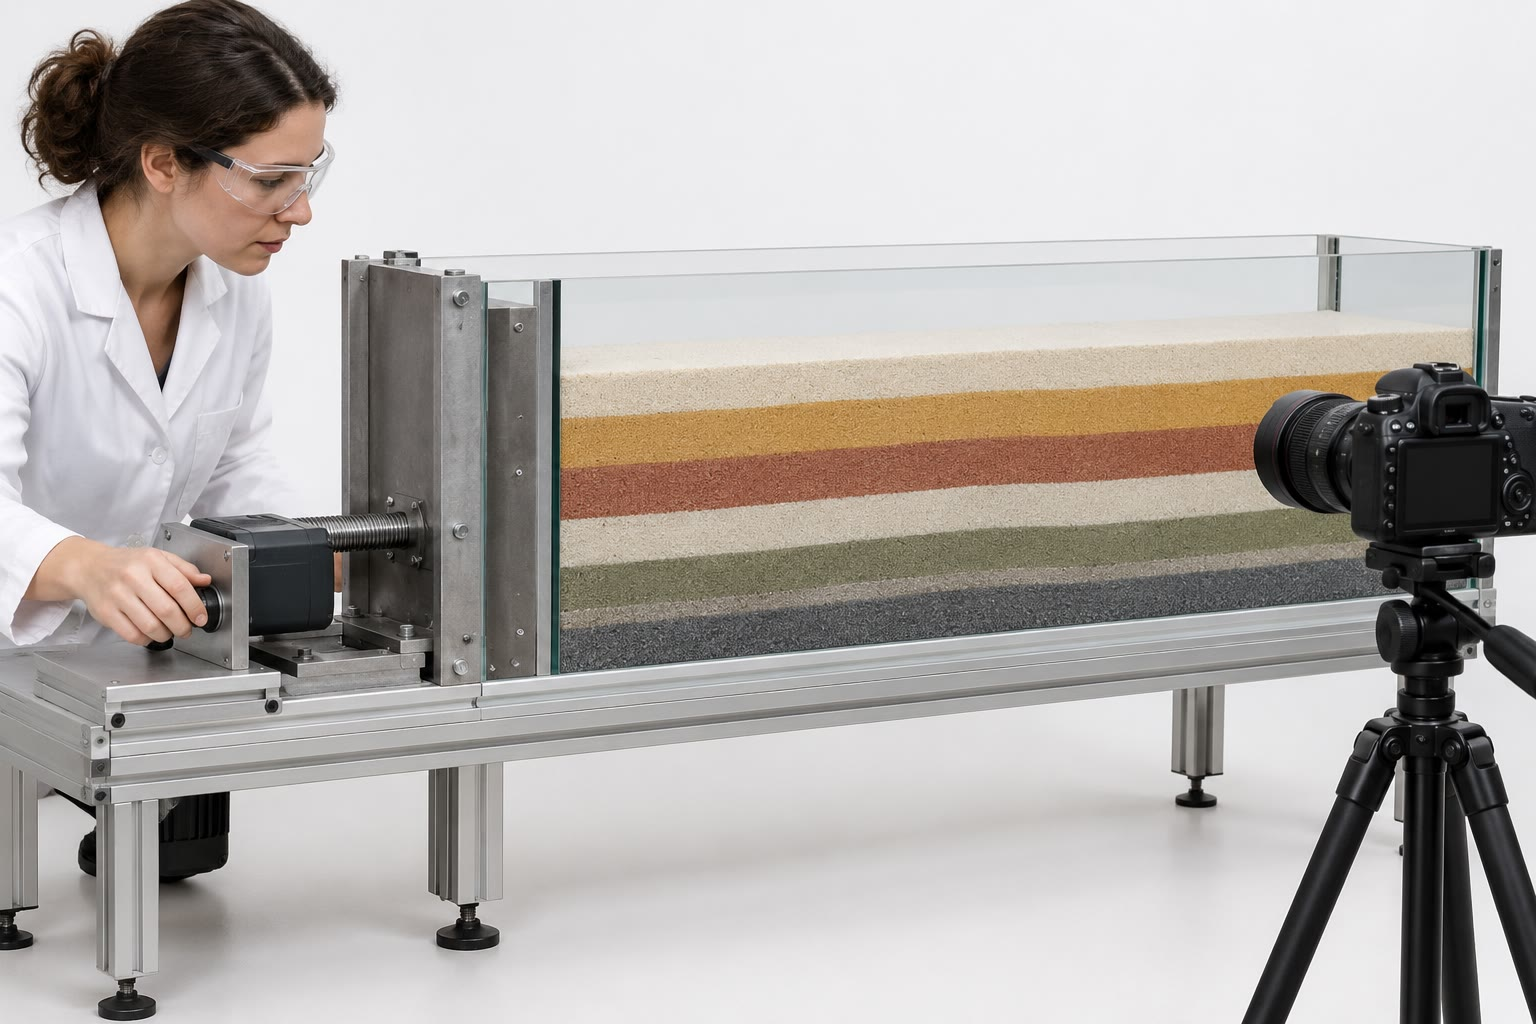
\includegraphics[width=\linewidth]{images/book5/ai/b3-sandbox-lab.jpg}

{\scriptsize Model kotak pasir sebelum pemendekan: lapisan pasir berwarna dalam
kotak berdinding kaca, dinding bermotor di sebelah kiri, kamera pada tripod
(ilustrasi buatan AI).}
\end{minipage}
\end{inthelab}
% ledger: dsd83:taper

\section{Baji nyata}\label{sec:b3:orogenic-wedges:real}

Di sabuk lipatan-dan-sesar dorong aktif di Taiwan bagian barat, kemiringan permukaan,
kemiringan décollement dan tekanan pori semuanya diketahui dari topografi,
penampang seismik dan sumur. Davis, Suppe, dan Dahlen menggunakannya untuk menyelesaikan
\omterm{thm:b3:orogenic-wedges:critical-taper}{persamaan taper kritis} untuk kekuatan baji dan mendapati $\mu = 1.03$
di dalam dan $\mu_b = 0.85$ pada dasar: gesekan Byerlee pada dasar, dan
baji yang lebih kuat daripada sesar-sesarnya sendiri, karena tidak semuanya berorientasi
mudah tergelincir. Dengan kedua koefisien ini, mereka mengubah taper teramati dari
baji aktif lain, di darat maupun di bawah laut, menjadi rasio tekanan pori, dan
mendapati bahwa semuanya di atas hidrostatik, sesuai dengan data pengeboran. Mereka juga mendapati
di mana teori berhenti berlaku: taper turun mendadak ketika baji tumbuh lebih tebal
daripada sekitar \qty{15}{km}, kedalaman tempat batuan kaya kuarsa menjadi plastis
untuk geoterm yang umum, dan dasar tidak lagi mematuhi hukum gesekan.
% ledger: dsd83:taper

Di front Alpen bagian barat, Jura adalah baji sesar dorong dengan sudut sempit
hanya 3 sampai \ang{4}. Décollement-nya sebagian besar terletak pada lapisan yang mengandung halit
berumur Trias, dan fluida di sana tidak bertekanan berlebih: kelemahan
garam saja sudah menjelaskan taper yang sempit. Di selatan Jura, tempat
lapisan Trias tidak mengandung halit, front yang sama memiliki taper 12 sampai
\ang{13}, dengan tumpukan irisan sesar dorong, meskipun tekanan fluida terukur
di sana tinggi. Di Alpen Tengah, analisis \omterm{def:b3:orogenic-wedges:critical-taper}{taper kritis} pada kemiringan permukaan
memberikan kekuatan dasar $\mu_b(1 - \lambda_b)$ (dengan suku
kohesi kecil) di bawah 0.1, dan bahkan 0.05 pada evaporit dan serpih dekat front,
meningkat ke arah belakang-pegunungan, dengan rasio tekanan pori di atas 0.54. Dasar
baji sering kali jauh lebih lemah daripada yang diberikan hukum Byerlee, oleh
jenis batuannya dan fluidanya.
% ledger: deville21:jura, vonhagke14:alps

\section{Fluks melalui baji}\label{sec:b3:orogenic-wedges:flux}

Baji pada \omterm{def:b3:orogenic-wedges:critical-taper}{taper kritisnya} tumbuh oleh akresi, dengan bentuk tetap: panjangnya
dan tingginya bertambah bersamaan. Erosi menghilangkan batuan dari permukaannya. Ketika
keduanya seimbang, baji mempertahankan ukurannya, dan batuan mengalir melalui baji itu.

\begin{proposition}[Keseimbangan fluks keadaan tunak]\label{prop:b3:orogenic-wedges:flux}
Sebuah baji dengan lebar $W$ sepanjang arah transpor menerima, per satuan panjang
sabuk, fluks akresi $F_a = v h$, dengan $v$ adalah
laju konvergensi dan $h$ tebal lapisan masuk di atas décollement. Ia
kehilangan fluks erosi $F_e = \bar e W$, dengan $\bar e$ adalah rata-rata
laju erosi pada permukaannya. Luas penampang melintangnya berubah dengan laju $F_a -
F_e$; pada keadaan tunak, $\bar e = vh/W$.
\end{proposition}

\begin{proof}
Dalam satuan waktu, panjang $v$ dari lapisan masuk, dengan tebal $h$, melewati
ke dalam baji melewati ujungnya, dan tebal $e(x)$ dihilangkan pada setiap
titik pada permukaannya; luasnya tetap, sehingga luas penampang
berubah sebesar $vh - \int_0^W e\,\mathrm dx = F_a - F_e$. Pada keadaan tunak
perubahan itu nol.
\end{proof}

Dengan $v = \qty{10}{mm/yr}$, $h = \qty{4}{km}$, dan $W = \qty{60}{km}$, laju
erosi yang diperlukan untuk keadaan tunak adalah $\qty{0.67}{mm/yr}$. Ekshumasi dalam
pengertian volume Tahun 2 adalah penghilangan batuan di atas batuan tertentu:
pada keadaan tunak, batuan mencapai permukaan dengan laju ketika erosi menurunkan
permukaan, dan baji membawanya naik dari kedalaman tempat batuan itu panas. Mengukur
seberapa cepat memerlukan jam yang dimulai pada suhu yang diketahui.

\section{Termokronologi}\label{sec:b3:orogenic-wedges:thermochronology}

\begin{definition}[Termokronologi, termokronometer]\label{def:b3:orogenic-wedges:thermochronology}
\emph{Termokronologi}\index{termokronologi} adalah penggunaan umur pendinginan radiometrik
untuk menentukan waktu saat suatu batuan melewati suhu tertentu, sehingga
sejarah termalnya dapat direkonstruksi. Sebuah
\emph{termokronometer}\index{termokronometer} adalah pasangan antara suatu mineral dan
metode penanggalan beserta suhu penutupannya: misalnya apatit
dengan metode (U--Th)/He, atau zirkon dengan jejak fisi.
\end{definition}

Tabel di bawah ini mengurutkan \omterm{def:b3:orogenic-wedges:thermochronology}{termokronometer} utama berdasarkan suhu penutupan;
kedalaman diperkirakan dengan asumsi suhu permukaan rata-rata \qty{10}{\celsius} dan
gradien seragam \qty{30}{\celsius/km}. Batuan yang mendingin ketika
diekshumasi melewati semuanya secara berurutan, dan umurnya bertambah dari metode suhu-rendah
ke metode suhu-tinggi. Fisika jejak fisi dan
difusi helium, yang menentukan suhu-suhu ini, dibahas dalam
\cref{ch:b3:advanced-geochronology}.
\begin{center}
\small
% ledger: sueoka19:closure
\begin{tabular}{lcc}
\hline
\omterm{def:b3:orogenic-wedges:thermochronology}{termokronometer} & suhu penutupan (\unit{\celsius}) & kedalaman (\unit{km}) \\
\hline
apatit (U--Th)/He & 50--80 & 1.3--2.3 \\
jejak fisi apatit & 90--120 & 2.7--3.7 \\
zirkon (U--Th)/He & 160--200 & 5.0--6.3 \\
jejak fisi zirkon & sekitar 280 & 9 \\
\textsuperscript{40}Ar/\textsuperscript{39}Ar pada biotit & 350--400 & 11--13 \\
\textsuperscript{40}Ar/\textsuperscript{39}Ar pada muskovit & sekitar 425 & 14 \\
U--Pb pada zirkon & di atas 900 & --- \\
\hline
\end{tabular}
\end{center}

Kedalaman-kedalaman ini hanyalah perkiraan awal, karena erosi mengubah geoterm.

\begin{proposition}[Geoterm keadaan tunak dengan erosi]\label{prop:b3:orogenic-wedges:geotherm}
Misalkan batuan naik dengan laju konstan $v$ melalui lapisan berketebalan $L$ yang
permukaannya ($z = 0$) dijaga pada suhu $T_s$ dan dasarnya pada $T_L$, tanpa
produksi panas. Suhu keadaan tunak adalah
\[
  T(z) = T_s + (T_L - T_s)\,\frac{1 - e^{-\mathrm{Pe}\,z/L}}{1 - e^{-\mathrm{Pe}}},
  \qquad \mathrm{Pe} = \frac{vL}{\kappa},
\]
dan gradien di permukaan adalah $\mathrm{Pe}/(1 - e^{-\mathrm{Pe}})$ kali
gradien konduktif $(T_L - T_s)/L$.
\end{proposition}

\begin{proof}
Partikel batuan pada kedalaman $z$ bergerak naik, menuju $z$ yang lebih kecil: suhu
yang dibawanya berubah sebagai $\partial T/\partial t - v\,\partial
T/\partial z$, dan persamaan difusi menjadi $\partial T/\partial t - v
T' = \kappa T''$. Pada keadaan tunak, $T'' = -(v/\kappa)T'$, sehingga $T' = C
e^{-vz/\kappa}$ dan $T = T_s + C(\kappa/v)(1 - e^{-vz/\kappa})$, yang memenuhi
$T(0) = T_s$. Dengan menetapkan $T(L) = T_L$ diperoleh $C$ dan rumusnya. Pada $z =
0$, $T' = (T_L - T_s)(\mathrm{Pe}/L)/(1 - e^{-\mathrm{Pe}})$.
\end{proof}

Untuk $\mathrm{Pe} \ll 1$ faktornya mendekati 1: konduksi mendominasi dan
geoterm tetap lurus. Untuk $v = \qty{1}{mm/yr}$ melintasi \qty{30}{km}, dengan
$\kappa = \qty{e-6}{m^2/s}$, $\mathrm{Pe} = 0.95$, dan gradien permukaan
naik dari 30 menjadi \qty{46}{\celsius/km}: isoterm-isoterm merapat ke
arah permukaan dan setiap \omterm{def:b3:orogenic-wedges:thermochronology}{termokronometer} menutup pada kedalaman yang lebih dangkal.
% ledger: england:kelvin, earle:settings

\begin{definition}[Hubungan umur--elevasi]\label{def:b3:orogenic-wedges:age-elevation}
\emph{Hubungan umur--elevasi}\index{hubungan umur--elevasi} suatu
\omterm{def:b3:orogenic-wedges:thermochronology}{termokronometer} adalah grafik umur pendinginan sampel yang dikumpulkan pada suatu
rentang elevasi, biasanya sepanjang lereng curam atau profil vertikal,
terhadap elevasinya.
\end{definition}

\begin{proposition}[Kemiringan hubungan umur--elevasi]\label{prop:b3:orogenic-wedges:age-elevation}
Misalkan batuan naik secara vertikal dengan laju konstan $v$ di bawah
topografi tunak, dan misalkan isoterm penutupan terletak pada elevasi $e(x) = e_0 +
f\,h(x)$, dengan $h(x)$ adalah elevasi permukaan dan $0 \le f < 1$. Sampel
yang dikumpulkan di permukaan pada elevasi $h$ memiliki umur $t = (h - e)/v$,
dan \omterm{def:b3:orogenic-wedges:age-elevation}{hubungan umur--elevasi} berupa garis lurus dengan kemiringan
\[
  \frac{\mathrm dh}{\mathrm dt} = \frac{v}{1 - f}.
\]
Untuk isoterm datar, $f = 0$ dan kemiringannya adalah laju ekshumasi.
\end{proposition}

\begin{proof}
Batuan yang kini berada di permukaan pada $x$ melintasi isoterm penutupan tepat
di bawahnya, pada elevasi $e(x)$, dan sejak itu telah naik $h - e$ dengan laju $v$:
$t = (h - e_0 - fh)/v = ((1 - f)h - e_0)/v$. Dengan demikian $\mathrm dt/\mathrm dh =
(1 - f)/v$.
\end{proof}

\begin{omfigure}
\begin{tikzpicture}
\begin{groupplot}[group style={group size=2 by 1, horizontal sep=1.7cm},
  omrecord, width=0.47\linewidth, height=0.45\linewidth, title style={font=\small},
  legend style={font=\scriptsize, legend cell align=left}]
\nextgroupplot[title={(a) umur--elevasi}, xlabel={umur apatit (U--Th)/He (\unit{Ma})},
  ylabel={elevasi di atas rata-rata (\unit{km})}, xmode=log, xmin=0.1, xmax=10,
  log ticks with fixed point, xtick={0.1,0.2,0.5,1,2,5,10}, ymin=-1, ymax=1]
% computed in figdata/bachelor-3/age_elevation.py
\addplot[black, thick, densely dotted] table[x=a30, y=h] {figdata/out/bachelor-3-age_elevation-ages.dat};
\addplot[red!70!black, thick, densely dashed] table[x=a10, y=h] {figdata/out/bachelor-3-age_elevation-ages.dat};
\addplot[omDef, thick] table[x=a03, y=h] {figdata/out/bachelor-3-age_elevation-ages.dat};
\nextgroupplot[title={(b) isoterm penutupan}, xlabel={jarak (\unit{km})},
  ylabel={elevasi di atas rata-rata (\unit{km})}, xmin=0, xmax=40, ymin=-3.3, ymax=1.2,
  legend style={at={(0.5,0.03)}, anchor=south, legend columns=2}]
\addplot[black!70, very thick] table[x=x, y=h] {figdata/out/bachelor-3-age_elevation-iso.dat};
\addlegendentry{permukaan}
\addplot[black, thick, densely dotted] table[x=x, y=e30] {figdata/out/bachelor-3-age_elevation-iso.dat};
\addlegendentry{\qty{3}{mm/yr}}
\addplot[red!70!black, thick, densely dashed] table[x=x, y=e10] {figdata/out/bachelor-3-age_elevation-iso.dat};
\addlegendentry{\qty{1}{mm/yr}}
\addplot[omDef, thick] table[x=x, y=e03] {figdata/out/bachelor-3-age_elevation-iso.dat};
\addlegendentry{\qty{0.3}{mm/yr}}
\end{groupplot}
\end{tikzpicture}

\par\smallskip{\small Ekshumasi tunak di bawah relief sinusoidal dengan
panjang gelombang \qty{20}{km} dan amplitudo \qty{1}{km}, untuk tiga laju,
gaya garis sama seperti pada legenda (b) (model orde pertama; lapisan setebal \qty{30}{km}, permukaan pada \qty{10}{\celsius},
\qty{30}{\celsius/km} tanpa erosi, $\kappa = \qty{e-6}{m^2/s}$, laju
penurunan suhu \qty{6.5}{\celsius/km}, suhu penutupan pada \qty{65}{\celsius}). (a) Umur terhadap
elevasi: kemiringannya adalah 0.59, 2.5, dan \qty{14}{mm/yr}, bukan 0.3, 1, dan 3.
(b) Isoterm \qty{65}{\celsius} semakin rapat mengikuti topografi, semakin
cepat ekshumasinya, karena isoterm itu naik lebih dekat ke permukaan.}\label{fig:b3:orogenic-wedges:age-elevation}
\end{omfigure}
% ledger: earle:settings, england:kelvin, ussa76:layers, sueoka19:closure

Isoterm tidak datar di bawah relief: permukaan lebih dingin di puncak
daripada di lembah, sebesar laju lapse atmosfer, tetapi jauh lebih kecil
dibandingkan batuan pada elevasi yang sama di bawah tanah, dan isoterm dangkal
mengikuti topografi dengan cara yang lebih lemah. Untuk topografi sinusoidal dengan
panjang gelombang $\Lambda$ dan laju lapse $\Gamma$, solusi orde pertama dari
persamaan tunak memberikan
\[
  f = \frac{(G_0 - \Gamma)\,e^{-mz_c}}{G(z_c)},\qquad
  m = \frac{v}{2\kappa} + \sqrt{\Bigl(\frac{v}{2\kappa}\Bigr)^2 +
  \Bigl(\frac{2\pi}{\Lambda}\Bigr)^2},
\]
dengan $z_c$ adalah kedalaman isoterm penutupan di bawah permukaan rata-rata,
$G_0$ gradien permukaan dan $G(z_c)$ gradien pada $z_c$ (diasumsikan;
skrip menguji hal itu). Gangguan itu meluruh dengan kedalaman sepanjang
jarak $1/m$, paling besar $\Lambda/2\pi$: \omterm{def:b3:orogenic-wedges:thermochronology}{termokronometer} suhu rendah,
yang menutup dangkal, paling peka terhadap relief. Gambar di atas menunjukkan pengaruh
untuk apatit (U--Th)/He.
% ledger: sueoka19:closure, ussa76:layers

Profil umur--elevasi hanya mengukur laju ekshumasi di tempat isoterm penutupan
datar di bawah relief. Di tempat lain, profil itu melebih-lebihkannya dengan faktor $1/(1 - f)$, yang mencapai
dua atau lebih untuk apatit (U--Th)/He pada relief dengan panjang gelombang \qty{20}{km}.
Umur dari beberapa \omterm{def:b3:orogenic-wedges:thermochronology}{termokronometer} pada sampel yang sama, dan model termal
relief, mengoreksinya.

\section{Latihan}

\begin{exercise}[$\star$]\label{exo:b3:orogenic-wedges:1}
Hitung $K$ dan rasio $\sigma'_1/\sigma'_3$ saat keruntuhan untuk baji dengan
$\phi = \ang{30}$.
\end{exercise}

\begin{exercise}[$\star$]\label{exo:b3:orogenic-wedges:2}
Baji kotak pasir berisi pasir kering ($\lambda = \lambda_b = 0$) memiliki $\mu = 0.6$
di dalamnya dan $\mu_b = 0.3$ pada alasnya. Hitung kemiringan permukaan kritisnya pada alas
datar, lalu pada alas yang miring \ang{3}.
\end{exercise}

\begin{exercise}[$\star$]\label{exo:b3:orogenic-wedges:3}
Dengan permukaan pada \qty{10}{\celsius} dan gradien \qty{30}{\celsius/km},
periksa kedalaman dalam tabel suhu penutupan untuk apatit
(U--Th)/He, jejak fisi apatit, dan jejak fisi zirkon. \omterm{def:b3:orogenic-wedges:thermochronology}{Termokronometer} mana
yang akan kamu pakai untuk penanggalan ekshumasi dari \qty{5}{km}?
\end{exercise}

\begin{exercise}[$\star$]\label{exo:b3:orogenic-wedges:4}
\omterm{def:b3:orogenic-wedges:thrust-geometry}{Tanjakan} setinggi \qty{2}{km} miring \ang{30}. Hitung panjang horizontalnya dan
panjangnya sepanjang kemiringan. Seberapa tinggi lapisan dinding gantung terangkat setelah
melewati seluruh \omterm{def:b3:orogenic-wedges:thrust-geometry}{tanjakan}, dan berapa slip yang membawa batas potongan lapisan
terbawah dari kaki \omterm{def:b3:orogenic-wedges:thrust-geometry}{tanjakan} ke datar atas?
\end{exercise}

\begin{exercise}[$\star\star$]\label{exo:b3:orogenic-wedges:5}
Dengan koefisien Taiwan, hitung kemiringan permukaan kritis pada alas
yang miring \ang{6} untuk $\lambda = \lambda_b = 0.4$ dan $0.9$. Apa akibat
kenaikan tekanan fluida bagi baji yang berada pada \omterm{def:b3:orogenic-wedges:critical-taper}{taper kritisnya}?
\end{exercise}

\begin{exercise}[$\star\star$]\label{exo:b3:orogenic-wedges:6}
\omterm{def:b3:orogenic-wedges:thrust-folds}{Lipatan tekukan-sesar} terletak di atas \omterm{def:b3:orogenic-wedges:thrust-geometry}{tanjakan} setinggi \qty{1.5}{km}; lapisan di atas
datar atas memiliki luas kelebihan \qty{6.0}{km^2}. Hitung besar slip. Seorang rekan
membaca lipatan yang sama sebagai \omterm{def:b3:orogenic-wedges:thrust-folds}{lipatan detasemen}, dengan lapisan terletak \qty{3.0}{km} di atas
décollement. Berapa pemendekan yang akan ia peroleh?
\end{exercise}

\begin{exercise}[$\star\star$]\label{exo:b3:orogenic-wedges:7}
Ambil $\mu = 0.6$ di dalam baji Jura (taper \ang{3.5}) dan baji di
selatannya (taper \ang{12.5}), $\lambda = 0.4$ hidrostatik di dalam keduanya, dan
kemiringan alas \ang{2} untuk keduanya. Hitung kekuatan basal $\mu_b(1 -
\lambda_b)$ yang dibutuhkan setiap taper, dan bandingkan dengan $0.85$ menurut hukum Byerlee
pada tekanan hidrostatik. Apakah hasilnya konsisten dengan décollement di
halit di bawah Jura?
\end{exercise}

\begin{exercise}[$\star\star$]\label{exo:b3:orogenic-wedges:8}
Batuan naik dengan laju \qty{1}{mm/yr} melalui lapisan setebal \qty{30}{km}, dari
\qty{910}{\celsius} di alasnya hingga \qty{10}{\celsius} di permukaan, dengan
$\kappa = \qty{e-6}{m^2/s}$. Hitung bilangan Péclet, gradien permukaan,
dan kedalaman isoterm \qty{65}{\celsius}. Bandingkan dengan kedalaman
tanpa erosi.
\end{exercise}

\begin{exercise}[$\star\star$]\label{exo:b3:orogenic-wedges:9}
Dua sampel dari lereng yang sama, pada 1200 dan \qty{2000}{m}, memiliki umur
(U--Th)/He apatit sebesar 3.4 dan \qty{4.6}{Ma}. Hitung laju ekshumasi semu
Model termal relief memberikan $f = 0.5$: berapa laju sebenarnya?
\end{exercise}

\begin{exercise}[$\star\star\star$]\label{exo:b3:orogenic-wedges:10}
Tunjukkan bahwa, untuk $\lambda = \lambda_b$, kemiringan permukaan kritis lenyap pada
kemiringan alas $\beta^* = \mu_b/K$ yang tidak bergantung pada $\lambda$. Hitung nilainya untuk
Taiwan. Apa yang terjadi pada baji yang alasnya miring lebih curam?
\end{exercise}

\begin{exercise}[$\star\star\star$]\label{exo:b3:orogenic-wedges:11}
Tunjukkan bahwa, untuk panjang gelombang yang sangat panjang dan ekshumasi yang sangat lambat, $f$ cenderung ke
$1 - \Gamma/G$, dengan $G$ adalah gradien seragam; evaluasi untuk $G =
\qty{30}{\celsius/km}$ dan $\Gamma = \qty{6.5}{\celsius/km}$. Berapa kemiringan
\omterm{def:b3:orogenic-wedges:age-elevation}{hubungan umur--elevasi} pada kondisi itu? Untuk $v = \qty{1}{mm/yr}$ dan nilai-nilai
latihan~8 ($z_c = \qty{1.21}{km}$, $G_0 = \qty{46.5}{\celsius/km}$,
$G(z_c) = \qty{44.7}{\celsius/km}$), hitung $f$ untuk panjang gelombang 5 dan
\qty{20}{km}.
\end{exercise}

\begin{exercise}[$\star\star\star$]\label{exo:b3:orogenic-wedges:12}
Sebuah baji tumbuh pada \omterm{def:b3:orogenic-wedges:critical-taper}{taper kritisnya} $\alpha + \beta$ melalui \omterm{def:b3:orogenic-wedges:accretion}{akresi frontal}
saja, tanpa erosi, dari fluks $F_a$. Tunjukkan bahwa lebarnya bertambah sebagai
$W = \sqrt{2F_at/\tan(\alpha + \beta)}$. Dengan $F_a = \qty{40}{km^2/Ma}$ dan
taper sebesar \ang{6}, seberapa lebar baji setelah \qty{2}{Ma}, dan berapa lama
yang dibutuhkan baji untuk mencapai \qty{60}{km}?
\end{exercise}

\section{Soal: Front baji Kestrel}

\begin{problem}[{Soal akhir pekan --- pemendekan, mekanika, fluks dan
ekshumasi baji sesar dorong rekaan}]
\label{pb:b3:orogenic-wedges:1}
% values: calc/ch10.py; critical_taper.py; age_elevation.py; fault_bend.py
Pegunungan Kestrel adalah front rekaan dari sebuah sabuk gunung, yakni sabuk
lipatan-dan-sesar dorong subaerial selebar \qty{60}{km} yang didorong dengan laju \qty{10}{mm/yr} di atas
depan-pegunungan yang lapisan sedimennya setebal \qty{4.0}{km} di atas serpih
décollement. Sesar dorong frontalnya mengikuti décollement \qty{4.5}{km} di bawah
permukaan, menaiki \omterm{def:b3:orogenic-wedges:thrust-geometry}{tanjakan} dengan kemiringan \ang{25}, lalu berjalan sepanjang \omterm{def:b3:orogenic-wedges:thrust-geometry}{bagian datar} atas
sedalam \qty{1.5}{km}. Di front, permukaan berada \qty{0.3}{km} di atas
permukaan laut dan décollement \qty{4.0}{km} di bawahnya; \qty{60}{km} di belakang
front, permukaan berada pada \qty{2.4}{km} dan décollement terletak
\qty{8.2}{km} di bawah permukaan laut. Ambil, seperti di Taiwan, $\mu = 1.03$ dan $\mu_b =
0.85$, massa jenis batuan \qty{2500}{kg/m^3}, massa jenis air \qty{1000}{kg/m^3}, dan
$g = \qty{9.81}{m/s^2}$.

\medskip\noindent\textbf{Bagian I --- Geometri sesar dorong.}
\begin{enumerate}
  \item Hitung tinggi \omterm{def:b3:orogenic-wedges:thrust-geometry}{tanjakan}, panjang horizontalnya, dan panjangnya
        sepanjang kemiringan.
  \item Seberapa jauh sebuah lapisan pada dinding gantung terangkat setelah
        melintasi seluruh \omterm{def:b3:orogenic-wedges:thrust-geometry}{tanjakan}?
  \item Di atas \omterm{def:b3:orogenic-wedges:thrust-geometry}{tanjakan}, sebuah lapisan di atas \omterm{def:b3:orogenic-wedges:thrust-geometry}{bagian datar} atas menunjukkan luas lebih
        sebesar \qty{16.5}{km^2} di atas tingkat regionalnya. Hitung pergeseran sesar.
  \item Berapa luas lebih yang kamu prediksi untuk lapisan yang lebih dangkal? Seandainya
        lipatan itu dibaca sebagai \omterm{def:b3:orogenic-wedges:thrust-folds}{lipatan detasemen} di atas décollement, dengan lapisan
        \qty{4.0}{km} di atasnya, berapa pemendekan yang akan ditemukan?
  \item Di belakang \omterm{def:b3:orogenic-wedges:thrust-geometry}{tanjakan}, sebuah penampang seismik menunjukkan \omterm{def:b3:orogenic-wedges:thrust-geometry}{dupleks} dari empat blok,
        masing-masing kini \qty{2.5}{km} panjangnya di sepanjang sesar dorong dasar, dipotong dari
        irisan sepanjang \qty{6.0}{km}. Hitung pemendekan yang ditampung oleh blok-blok itu, lalu
        bandingkan dengan pergeseran pada \omterm{def:b3:orogenic-wedges:thrust-geometry}{tanjakan} frontal.
  \item Blok-blok itu terbentuk berurutan. Yang mana paling muda, dan mengapa sesar dorong
        atapnya terlipat?
\end{enumerate}

\medskip\noindent\textbf{Bagian II --- Taper.}
\begin{enumerate}[resume]
  \item Hitung kemiringan permukaan $\alpha$, kemiringan dasar $\beta$, dan
        taper.
  \item Hitung tebal baji \qty{60}{km} di belakang front. Apakah teori baji Coulomb
        dapat digunakan?
  \item Hitung $K$. Berapa kemiringan permukaan yang dimiliki baji kering di atas dasar ini?
  \item Berapa kemiringan permukaan yang dimiliki baji dengan tekanan fluida hidrostatik
        di dalam baji dan pada dasarnya? Apakah baji konsisten dengan keadaan itu?
  \item Selesaikan \omterm{thm:b3:orogenic-wedges:critical-taper}{persamaan taper kritis} untuk $\lambda = \lambda_b$.
  \item Hitung tegangan vertikal, tekanan fluida, dan tekanan hidrostatik
        di dasar baji \qty{60}{km} di belakang front.
  \item Drainase menurunkan $\lambda$ menjadi 0.7. Hitung kemiringan permukaan kritis
        yang baru. Bagaimana baji meresponsnya?
\end{enumerate}

\medskip\noindent\textbf{Bagian III --- Fluks.}
\begin{enumerate}[resume]
  \item Hitung fluks akresi per kilometer sabuk.
  \item Berapa laju erosi rata-rata yang menjaga baji tetap dalam keadaan tunak?
  \item Hitung volume dan massa batuan yang tererosi per tahun dari
        \qty{100}{km} sabuk itu.
  \item Jika erosi berhenti, seberapa cepat baji akan melebar pada awalnya?
  \item Jika separuh lapisan masuk mengalami \omterm{def:b3:orogenic-wedges:accretion}{underplating tektonik} di bawah bagian belakang
        baji, bukan diakresikan di depannya, apakah laju erosi rata-rata keadaan tunak berubah?
        Di mana erosi akan terkonsentrasi?
\end{enumerate}

\medskip\noindent\textbf{Bagian IV --- Jam.}
Ambil lapisan setebal \qty{30}{km}, bersuhu \qty{10}{\celsius} di permukaan rata-rata
(\qty{2.0}{km} di atas permukaan laut) dan \qty{910}{\celsius} di dasarnya, $\kappa
= \qty{e-6}{m^2/s}$, suhu penutupan apatit (U--Th)/He sebesar \qty{65}{\celsius},
(U--Th)/He, laju penurunan suhu \qty{6.5}{\celsius/km}, dan relief dengan
panjang gelombang \qty{20}{km}. Lima sampel yang dikumpulkan pada satu sisi lembah memberikan:
\begin{center}
\small
\begin{tabular}{lccccc}
\hline
elevasi (\unit{km}) & 1.30 & 1.65 & 2.00 & 2.35 & 2.70 \\
umur apatit (U--Th)/He (\unit{Ma}) & 1.60 & 1.83 & 2.07 & 2.30 & 2.54 \\
\hline
\end{tabular}
\end{center}
\begin{enumerate}[resume]
  \item Dengan laju erosi pada pertanyaan 15 sebagai laju ekshumasi, hitung
        \omterm{def:b3:lithosphere-thermal-models:peclet}{bilangan Péclet termal} dan gradien permukaan.
  \item Hitung kedalaman isoterm penutupan di bawah permukaan rata-rata, dan
        gradiennya di sana.
  \item Dengan isoterm penutupan yang datar, berapa umur yang dimiliki sampel pada elevasi
        rata-rata? Bandingkan dengan data.
  \item Hitung $m$ dan faktor defleksi $f$.
  \item Cocokkan garis lurus pada data umur--elevasi. Laju ekshumasi semu apa yang
        diberikan oleh kemiringannya?
  \item Koreksi hasil itu terhadap defleksi isoterm.
  \item Bandingkan dengan Bagian III, dan berikan laju ekshumasi baji
        Kestrel.
\end{enumerate}
\end{problem}
